\documentclass[11pt,a4paper]{article}
\usepackage[margin=24mm,headheight=15pt]{geometry}
\usepackage[T1]{fontenc}
\usepackage{lmodern}
\usepackage{graphicx}
\usepackage{booktabs,tabularx,longtable,array}
\usepackage{amsmath}
\usepackage{xcolor,listings,float,fancyhdr,hyperref}
\definecolor{accent}{HTML}{17566A}
\definecolor{codebg}{HTML}{F3F6F8}
\hypersetup{colorlinks=true,linkcolor=accent,urlcolor=accent,citecolor=accent,
  pdftitle={Rate-Limited Sender Functionality in picoquic},
  pdfauthor={Aryan Bokolia; Affan Arshad; Soumyadeep Raj; Kevin Shiju George; Aryan Sanjay palimkar}}
\pagestyle{fancy}
\fancyhf{}
\fancyhead[L]{\small Project 16: Rate-Limited CUBIC}
\fancyhead[R]{\small Project report}
\fancyfoot[C]{\thepage}
\setlength{\parindent}{0pt}
\setlength{\parskip}{6pt}
\setlength{\emergencystretch}{2em}
\renewcommand{\arraystretch}{1.15}
\lstset{basicstyle=\ttfamily\footnotesize,backgroundcolor=\color{codebg},
  frame=single,rulecolor=\color{black!12},breaklines=true,columns=fullflexible,
  keepspaces=true,showstringspaces=false,xleftmargin=3pt,xrightmargin=3pt}
\newcommand{\code}[1]{\texttt{\detokenize{#1}}}
% Generated exclusively from the fresh logs by analyze_results.py.
\newcommand{\BaselineCommit}{5a4eba475555}
\newcommand{\ImplementationCommit}{80c9186fd466}
\newcommand{\WindowChange}{98.90}
\newcommand{\BulkChange}{2.96}
\newcommand{\ObservedRateFlight}{3426}
\newcommand{\RateBaselineThroughput}{0.189}
\newcommand{\RateBaselineCwnd}{15.000}
\newcommand{\RateRliThroughput}{0.189}
\newcommand{\RateRliCwnd}{29.834}
\newcommand{\BulkBaselineThroughput}{17.097}
\newcommand{\BulkBaselineCwnd}{504.391}
\newcommand{\BulkRliThroughput}{17.603}
\newcommand{\BulkRliCwnd}{286.778}
\newcommand{\TestCountSummary}{baseline: 562 + 105 subtests; rli: 563 + 105 subtests}


\begin{document}
\hypersetup{pageanchor=false}
\begin{titlepage}
\centering
\vspace*{10mm}
{\Large\color{accent} PROJECT REPORT}\par
\vspace{7mm}
{\large Project \#16}\par
\vspace{10mm}
{\Huge\bfseries Implementation of\\[3mm] Rate-Limited Sender\\[3mm] Functionality in picoquic}\par
\vspace{8mm}
{\Large CUBIC congestion control: implementation and tests}\par
\vspace{12mm}
\rule{0.8\textwidth}{0.7pt}\par
\vspace{7mm}
{\large Team members}\par
\vspace{3mm}
{\Large\bfseries Aryan Bokolia\\[2mm]
Affan Arshad\\[2mm]
Soumyadeep Raj\\[2mm]
Kevin Shiju George\\[2mm]
Aryan Sanjay palimkar}\par
\vspace{7mm}
{\large 7 November 2026}\par
\vspace{6mm}
{\normalsize Baseline revision: \texttt{\BaselineCommit}\\
Implementation revision: \texttt{\ImplementationCommit}}\par
\vfill
\end{titlepage}
\pagenumbering{roman}
\hypersetup{pageanchor=true}

\section*{Abstract}
\addcontentsline{toc}{section}{Abstract}
This project adds an optional Rate-Limited Increase (RLI) mode to CUBIC in picoquic.
The congestion window, or cwnd, limits outstanding data.
Baseline CUBIC restricts window growth when the application cannot fill that window.
RLI allows growth after acknowledgements and caps it using the flight-size history of each path.

Both source revisions passed the registered Linux test suites.
The implementation also passed the focused \code{cubic_rli} test.
The experiments include twelve single-flow runs and six runs with two competing flows.
Each configuration has three repetitions.

In the rate-limited workload, the final cwnd increased from 15 KiB to 30 KiB.
The mean time-weighted cwnd increased by \WindowChange\%.
Throughput stayed near 0.190 Mbit/s because the application supplied limited data.
Mean bulk throughput was \BulkBaselineThroughput{} Mbit/s for baseline and \BulkRliThroughput{} Mbit/s for RLI, a \BulkChange\% difference.
The competing-flow tests measured similar combined throughput in both modes.
These results describe the tested workloads and the implemented growth limits.

\tableofcontents
\clearpage
\pagenumbering{arabic}

\section{Project details and objectives}
The project implements rate-limited sender functionality in picoquic CUBIC.
Linux network namespaces provide the test network.
The reference is draft-ietf-ccwg-ratelimited-increase-11, an IETF Congestion Control Working Group document \cite{rli}.

The work compares baseline CUBIC with the RLI implementation.
The main checks cover window growth, growth limits, congestion responses, and operation with RLI disabled.
Logs and graphs show how each version behaves under the same workload.

\begin{longtable}{>{\raggedright\arraybackslash}p{0.07\textwidth}>{\raggedright\arraybackslash}p{0.37\textwidth}>{\raggedright\arraybackslash}p{0.48\textwidth}}
\toprule Step & Requirement & Evidence\\\midrule
\endhead
1 & Install picoquic on Linux without a VM & Native Linux builds and saved build logs.\\
2 & Study congestion-control algorithms & Architecture notes and the file map in Section~\ref{sec:files}.\\
3 & Set up a Linux netns dumbbell & Connectivity and queue checks for the single-flow path and two-pair dumbbell.\\
4 & Run baseline CUBIC and plot cwnd & Three rate-limited runs and three bulk runs.\\
5 & Identify the required CUBIC changes & Flight tracking, growth limits, recovery handling, and logging design.\\
6 & Implement RLI for CUBIC & Source changes and the focused regression test.\\
7 & Repeat the experiments with RLI & Six matching single-flow runs and their cwnd plots.\\
8 & Validate the results & Trace checks, measured comparisons, and saved test outputs.\\
\bottomrule
\end{longtable}

\section{Background: QUIC, picoquic, and CUBIC}
\subsection{QUIC and picoquic}
QUIC is a secure transport protocol carried over UDP.
It supports multiple streams, connection establishment, and migration between network paths \cite{quic}.
QUIC loss recovery and congestion control are specified separately \cite{quiccc}.
The application supplies data, and QUIC sends it in packets.
Acknowledgements and congestion signals affect how much data the sender can keep outstanding.

picoquic is a C implementation of QUIC with demonstration programs, congestion-control callbacks, logging, and tests \cite{picoquic}.
This project changes its userspace CUBIC implementation.
The demo option \code{-G cubic} selects that algorithm.
Changing the Linux TCP congestion-control setting does not select the algorithm for a picoquic connection.

\subsection{Terms and units}
\begin{tabularx}{\textwidth}{lX}
\toprule Term & Meaning\\\midrule
\code{cwnd} / \code{cwin} & Congestion window in bytes. The code uses the name \code{cwin}.\\
FlightSize & Outstanding data, tracked by \code{bytes_in_transit}.\\
\code{maxFS} & Flight-size history used to set the RLI growth limit.\\
ACK & Acknowledgement of previously sent data.\\
RTT & Round-trip time between a transmission and its acknowledgement.\\
Throughput & Application bytes per unit time. This report uses decimal Mbit/s.\\
KiB & 1,024 bytes. A 15 KiB window contains 15,360 bytes of permitted capacity.\\
\bottomrule
\end{tabularx}

\subsection{CUBIC and application limitation}
CUBIC uses a cubic time-based window target in congestion avoidance.
It also keeps a Reno-friendly estimate \cite{cubic}.
The picoquic implementation contains Slow Start, recovery, HyStart-related behavior, and congestion avoidance in \path{picoquic/cubic.c}.
Its constants and recovery decisions come from that source revision.
They are not assumed to match every detail of Linux TCP CUBIC.

A sender is application-limited when the application provides less data than the congestion window permits.
A larger window cannot create more application data.
Bytes in flight can therefore remain below cwnd throughout a transfer.
The height of a cwnd curve does not, by itself, show a throughput gain.

\section{Baseline definition and observed behavior}
The baseline is the unchanged pre-RLI revision \texttt{\BaselineCommit}.
Its source was extracted with \code{git archive} and built in \path{.local-deps/report-baseline/build/}.
The implementation revision is \texttt{\ImplementationCommit}.
The two versions use separate executables.
The saved evidence includes source revisions and executable SHA-256 hashes.

Baseline CUBIC uses sender-limited timestamps to decide whether to grow cwnd.
Its Slow Start helper also checks whether the connection was blocked by cwnd.
One relevant condition is:
\begin{lstlisting}[language=C]
path_x->last_time_acked_data_frame_sent >
    path_x->last_sender_limited_time
\end{lstlisting}
The low-rate application does not fill the window.
Baseline cwnd therefore remains at its initial value:
\[
  \mathrm{initial\_cwnd} = 10\times 1536 = 15360\;\mathrm{bytes}
  = 15\;\mathrm{KiB}.
\]
These constants are defined in \path{picoquic/picoquic_internal.h}.
The value 1536 is the compile-time maximum packet-size constant used for the initial window.
It differs from the 1200-byte application frame and the negotiated path MTU.

\section{RLI design and the reference draft}
The draft defines flight-history tracking and a limit on window growth \cite{rli}.
The implementation applies these rules:
\begin{lstlisting}
initialize:        maxFS = initial_cwnd
on flight change:  maxFS = max(maxFS, bytes_in_transit)
after reduction:   maxFS = 0
on ACK:           compute candidate congestion window
                  apply an RLI growth limit
                  update pacing and log state
\end{lstlisting}
The implemented limits are:
\[
 L_{\mathrm{SS}} = 2\,\mathrm{maxFS},\qquad
 L_{\mathrm{CA}} = \mathrm{maxFS} + \mathrm{send\_mtu}.
\]
Slow Start adds acknowledged bytes before applying the cap.
Congestion avoidance computes the CUBIC/Reno candidate, then applies the \code{maxFS + send_mtu} ceiling.

Section 3 of the draft gives the additive congestion-avoidance expression.
Section 4.5 applies the Section 3 rules to CUBIC \cite{rli}.
It retains the exclusion of application-limited time from the CUBIC epoch.
This implementation uses the explicit additive expression as a conservative ceiling.
The draft also defines the limit through an algorithm's growth over one acknowledged flight.
A different time-dependent CUBIC interpretation would need its own derivation and tests.
The checks here validate the stated additive ceiling.
They do not provide independent standards certification.

The cap limits growth without forcing a further window reduction.
If a candidate exceeds both the previous cwnd and the limit, the code selects \(\max(\mathrm{previous\_cwnd},L)\).
Congestion responses and window validation remain separate mechanisms.

\subsection{Why the window changes from 15 KiB to 30 KiB}
At startup, \code{maxFS} is initialized to 15,360 bytes.
This initial value applies even when the measured flights are smaller.
It stays unchanged in the rate-limited runs.
ACKs allow Slow Start growth up to \(2\times15360=30720\) bytes, or 30 KiB.
Further small bursts cannot raise this ceiling unless the sender observes a larger flight.

The largest observed flight in these traces was \ObservedRateFlight{} bytes.
The 15 KiB history value therefore includes the initialization floor.
It does not mean the application sent 15 KiB at once.
RLI increases permitted capacity while the application continues to supply limited data.
These experiments do not measure the speed of a later burst after an idle period.

\section{Implementation and changed files}\label{sec:files}
\begin{longtable}{>{\raggedright\arraybackslash}p{0.42\textwidth}>{\raggedright\arraybackslash}p{0.51\textwidth}}
\toprule File & Change\\\midrule
\endhead
\path{picoquic/picoquic_internal.h} & Adds per-path RLI state and the flight-tracking helper declaration. The fields include \code{rli_max_flight_size} and \code{rli_cwin_limit}.\\
\path{picoquic/sender.c} & Calls \code{picoquic_update_max_flight_size()} when send and dequeue operations change flight size.\\
\path{picoquic/cubic.c} & Adds the option, state initialization, growth caps, recovery handling, and cleanup.\\
\path{picoquic/logwriter.c} & Adds RLI values to binary congestion records.\\
\path{loglib/qlog.c} & Converts the added binary values to qlog metrics.\\
\path{loglib/qlog_fns.c} & Writes RLI metrics through the direct qlog path.\\
\path{picoquictest/congestion_test.c} & Adds the focused \code{cubic_rli} test.\\
\path{picoquictest/picoquictest.h} & Declares the test.\\
\path{picoquic_t/picoquic_t.c} & Registers the test in the Linux runner.\\
\path{UnitTest1/unittest1.cpp} & Registers the Visual Studio test. This verification did not run that platform.\\
\path{plot_cwnd.py} & Reconstructs qlog metric values for each path and plots cwnd, flight size, and RLI state.\\
\path{experiments/run_comparison.sh} & Runs the main comparison and saves logs, plots, and metadata.\\
\path{experiments/validate_rli.py} & Checks observed trace rules and compares measured results.\\
\path{topology/setup.sh}, \path{check.sh}, \path{cleanup.sh} & Create, check, and remove the single-flow topology.\\
\path{topology/setup_dumbbell.sh}, \path{topology/check_dumbbell.sh} & Create and check the full two-pair dumbbell.\\
\bottomrule
\end{longtable}

\subsection{Implementation decisions}
The code updates flight history at packet-accounting points.
An ACK snapshot alone can miss an earlier flight peak.
After a congestion reduction, later flight measurements rebuild the history.
The focused test checks explicit congestion notification (ECN), timeout, accepted loss, and live send/dequeue accounting.

Spurious-loss correction restores CUBIC state without restoring flight history from before the reduction.
The Reno-friendly shadow window stays within the permitted cwnd.
This prevents a stored excessive target from causing later growth.
The code retains exclusion of application-limited time from the CUBIC epoch.

The option \code{-G cubic -H rli=on} enables RLI.
Without it, CUBIC follows the legacy path.
A separate DCUBIC initializer keeps RLI disabled in that shared implementation.
The cap calculation saturates at the unsigned integer maximum to prevent overflow.
The focused test does not separately exercise the overflow boundary.

\subsection{Runtime workflow}
\begin{enumerate}
\item The application supplies media frames or requests the bulk file.
\item picoquic sends packets and updates outstanding bytes and \code{maxFS}.
\item ACKs and congestion notifications call the CUBIC algorithm.
\item With RLI enabled, CUBIC computes a candidate window and applies the growth limit.
\item Loss, ECN, or timeout recovery resets the history after a window reduction.
\item qlog and performance CSV files record the connection state and transfer measurements.
\item Python scripts reconstruct metric values, check traces, and create graphs and comparisons.
\end{enumerate}

\section{Linux verification and test selection}
Verification ran on native Ubuntu 26.04 LTS with an x86-64 processor and kernel 7.0.0-38-generic.
The compiler was GCC 15.2.0, and the build tool was CMake 4.2.3.
The host virtualization check returned \code{none}.
Both versions used RelWithDebInfo builds, the same local picotls source, and the same OpenSSL headers and libraries.
The baseline build explicitly includes the OpenSSL multiarch directory to match the current build settings.

\subsection{Registered regression suites}
Both versions passed the registered CTest entries, \code{picoquic_ct} and \code{picohttp_ct}.
Their internal results were:
\begin{center}
\begin{tabular}{lrrr}\toprule
Revision & picoquic subtests & picohttp subtests & Failures\\\midrule
Baseline & 562 & 105 & 0\\
RLI implementation & 563 & 105 & 0\\\bottomrule
\end{tabular}
\end{center}
The registered commands use \code{-n -r}.
These options suppress debug output and permit retries of failed cases.
The saved logs report zero failures.
The default suites do not cover every optional stress test, fuzz configuration, interoperability test, or sanitizer build.

\subsection{Focused RLI checks}
The \code{cubic_rli} test contains these behavior checks:
\begin{enumerate}
\item Initialization of \code{maxFS}.
\item Tracking of peak flight size.
\item Slow Start growth capped at twice the history.
\item Repeated limited bursts with the same ceiling.
\item A larger flight raising the ceiling.
\item ECN reduction and history reset.
\item Live send and dequeue accounting.
\item Spurious recovery retaining post-reduction history.
\item A growth cap that does not force another reduction.
\item Timeout reset and the minimum-window response.
\item Isolated loss filtering and accepted-loss reset.
\item Reno-friendly growth below the congestion-avoidance limit.
\item A large CUBIC candidate capped at that limit.
\item Exclusion of application-limited time from the epoch.
\item Legacy behavior in Slow Start and congestion avoidance with RLI disabled.
\end{enumerate}
These assertions belong to one registered test.
They are not separate CTest cases.

\subsection{Network test cases}
The network experiments use two workloads:
\begin{description}
\item[Rate-limited stream:] The application sends 400 frames of 1200 bytes at 20 frames/s.
This gives 480,000 application bytes over about 20 seconds, targeting 192 kbit/s.
The quicperf scenario is:
\begin{lstlisting}
=rli:s20:n400:1200:G20:I1200;
\end{lstlisting}
\item[Bulk control:] A 20 MiB file, or 20,971,520 bytes, keeps the sender supplied with data.
The connection CSV can include protocol framing beyond the file size.
\end{description}
Each workload runs three times in each mode, giving twelve single-flow runs.
The order changes in repetition two to reduce ordering bias.
Three repetitions show consistency within this test setup.
They do not establish statistical significance across network conditions.

\section{Topology and experiment controls}
The single-flow comparison uses four Linux network namespaces:
\begin{lstlisting}
rls-client -- rls-r1 == 20 Mbit/s == rls-r2 -- rls-server
\end{lstlisting}
The client address is \code{10.10.1.2}, and the server address is \code{10.10.2.2}.
The router link uses \code{10.10.12.0/30}.
Linux netem applies 25 ms delay, a 20 Mbit/s rate, and a 1000-packet queue limit in each direction.
The base RTT is about 50 ms, plus processing and queueing.

The scripts use \code{unshare} with Linux user, network, and mount namespaces.
A private tmpfs on \code{/run} stores isolated namespace handles.
The experiments do not use a virtual machine.
Topology checks confirm the namespaces, end-to-end connectivity, and both netem queue disciplines.
The first ping can include neighbour-resolution delay.
The later samples, near 50 ms, better represent the base path than the three-ping average.

Both revisions use the same topology, certificates, application settings, and build settings.
The analysis uses server qlogs because the server sends the application data.
Source revisions and binary hashes identify the tested executables.

The additional tests use two client/server pairs across the same bottleneck:
\begin{lstlisting}
client 1 --- r1 ===== shaped link ===== r2 --- server 1
client 2 ---/                            \--- server 2
\end{lstlisting}
The second client uses \code{10.10.3.2}, and the second server uses \code{10.10.4.2}.
Both connections start together, and each transfers 20 MiB.
This dumbbell has six namespaces.
Each mode runs three times with the same compiled revisions as the single-flow tests.
The two experiment sets are reported separately.

\section{Experimental results}
The tables show averages from all three repetitions.
The graph pages show repetition 1 only for each workload and mode.
The other repetitions remain in the saved results.
\begin{table}[H]\centering\small
\begin{tabular}{lrrrrr}\toprule
Mode & Final cwnd & Avg. cwnd & Rate & Time & Retrans.\\
 & (KiB) & (KiB) & (Mbit/s) & (s) & \\\midrule
baseline & 15.00 & 15.00 & 0.190 & 20.191 & 0.0 \\
rli & 30.00 & 29.81 & 0.190 & 20.191 & 0.0 \\
\bottomrule\end{tabular}
\caption{Rate-limited workload: means of all three repetitions. Time uses the server connection duration.}\end{table}
\begin{table}[H]\centering\small
\begin{tabular}{lrrrrr}\toprule
Mode & Final cwnd & Avg. cwnd & Rate & Time & Retrans.\\
 & (KiB) & (KiB) & (Mbit/s) & (s) & \\\midrule
baseline & 294.59 & 213.42 & 17.732 & 9.462 & 0.0 \\
rli & 264.92 & 234.48 & 17.950 & 9.347 & 0.0 \\
\bottomrule\end{tabular}
\caption{Bulk workload: means of all three repetitions. Time uses the server connection duration.}\end{table}

\begin{figure}[H]\centering
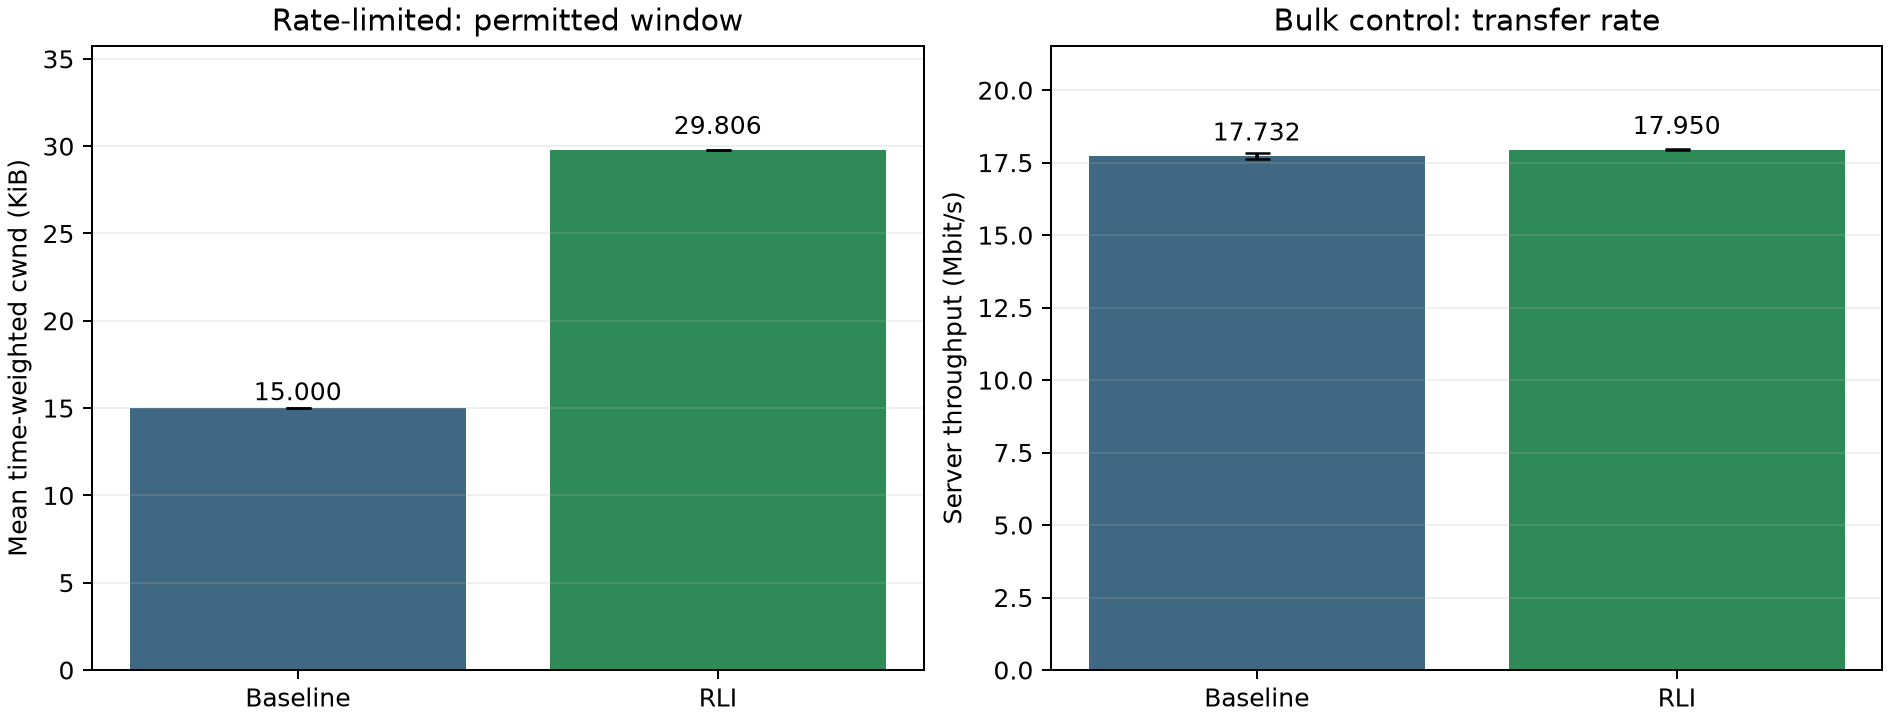
\includegraphics[width=\textwidth]{plots/overview.png}
\caption{Three-run means with sample standard-deviation error bars.
Left: time-weighted cwnd for the rate-limited workload.
Right: throughput for the bulk workload.}
\end{figure}

\subsection{Rate-limited window growth}
Mean time-weighted cwnd was \RateBaselineCwnd{} KiB for baseline and \RateRliCwnd{} KiB for RLI.
The increase was \WindowChange\%.
The final cwnd was 15 KiB for baseline and 30 KiB for RLI.
RLI allowed ACK-driven growth and then held the window at its ceiling.

Mean throughput was \RateBaselineThroughput{} Mbit/s for baseline and \RateRliThroughput{} Mbit/s for RLI.
Application supply limited both connections.
These measurements do not show more delivered data or faster restart after an idle period.

\subsection{Bulk-control results and metric definitions}
Mean bulk throughput was \BulkBaselineThroughput{} Mbit/s for baseline and \BulkRliThroughput{} Mbit/s for RLI.
The observed difference was \BulkChange\%.
With three local runs, this difference does not establish a statistically significant speed gain.
Scheduling, queueing, ACK timing, and CUBIC dynamics can affect the measurements.

The tables use connection duration from the server performance CSV.
The qlog metric span is stored separately in \path{measurements.csv}.
Throughput uses the server's sent-byte count divided by its connection duration, expressed in decimal Mbit/s.
Cwnd statistics use reconstructed metric snapshots with left-step time weighting.
The cap fraction includes the logger's initial zero-flag interval.
The generic helper starts that fraction at the first explicit flag observation.
This adjustment changes cap-duration statistics, but leaves cwnd and throughput measurements unchanged.
Final cwnd is retained window state at transfer completion.
It does not represent outstanding data at that time.

\subsection{Two competing flows}
\begin{table}[H]\centering\small
\begin{tabular}{lrrrrr}\toprule
Mode & Flow 1 & Flow 2 & Combined & Jain index & Retrans.\\
 & (Mbit/s) & (Mbit/s) & (Mbit/s) & & \\\midrule
baseline & 8.974 & 8.822 & 18.665 & 0.9995 & 450.0 \\
rli & 8.513 & 8.420 & 18.625 & 0.9998 & 432.7 \\
\bottomrule\end{tabular}
\caption{Two-flow dumbbell: means of all three repetitions. Retransmissions are the mean total across both flows.}\end{table}
Mean combined throughput was 18.665 Mbit/s for baseline and 18.625 Mbit/s for RLI (-0.22\%).
The common interval starts at client launch and ends when both clients exit.
It excludes the later wait for server shutdown.
Each flow rate uses that server's own connection interval.
The sum of those rates therefore differs from the combined wall-time rate.
The Jain index uses the two per-connection rates.
Values closer to one mean a more even split across these connection lifetimes.
This measure does not show instantaneous fairness or fairness against other congestion algorithms.

Both connections use the same congestion-control mode.
These tests do not compare fairness between different algorithms.
The checks confirm transfer byte counts at both sender and receiver.
Each RLI connection also passes the observed trace checks.

\section{Graph reading guide and validation results}
The detailed graphs use seconds on the x-axis and KiB on the y-axis.
Blue shows cwnd, and grey shows bytes in flight.
The RLI plots also show \code{maxFS}, the growth limit, and cap-active markers.
The window can overlap the limit line when their values match.

The rate-limited graph pair shows whether limited application data permits bounded window growth.
The bulk graph pair shows operation when the sender has continuous data.
The workload differs between these sets, so window height alone is not a useful performance comparison.
At transfer completion, bytes in flight can reach zero while cwnd retains its last value.

All six main RLI traces passed the validator.
The six RLI connections in the competing-flow tests also passed.
The main rate-limited runs must show an active cap.
The main bulk runs must show a window reduction with a flight-history reset.
The analysis also checks qlog JSON, a single sender path, transfer sizes, throughput arithmetic, and absent RLI metrics in baseline traces.

Both builds and their registered suites passed.
The focused test and measured traces support the stated growth limits under the tested conditions.

\subsection{Limitations and further tests}
The experiments use one bottleneck capacity, one base delay, and three repetitions per configuration.
Further tests should cover bursts after idle, receiver flow-control limits, longer idle periods, and changing delay.
Other useful cases include competition with different congestion algorithms, multiple paths, and deliberately injected loss or ECN.
Unit tests of congestion notifications do not replace those network experiments.

Qlog snapshots can miss intermediate flight peaks.
The validator therefore checks only observable trace properties.
Per-path storage alone does not prove multipath correctness.
Overflow boundary cases were not separately tested.
The fixed additive ceiling does not resolve every interpretation of the draft's general CUBIC limit.
Long-term window decay and RFC 7661 window validation remain outside this work.
More runs and network conditions are needed to estimate broader performance effects.

\section{Conclusion}
RLI permits the rate-limited CUBIC window to grow from 15 KiB to a bounded 30 KiB in these experiments.
The application rate remains essentially unchanged.
Both revisions pass the registered test suites, and the RLI trace checks pass for both experiment sets.
Bulk and competing-flow measurements show the transfer rates under greater offered load.
Broader performance and conformance claims require further tests and independent review.

\section{Reproduction and evidence files}
Run these commands from the repository root.
The collection scripts save raw measurements, and the analysis scripts create tables and graphs.
\begin{lstlisting}[language=bash]
cd /home/aryy_02/Desktop/OSNT_Project
python3 "results/run_tests.py"
unshare --user --map-root-user --net --mount \
  bash "results/run_experiments.sh"
.venv/bin/python "results/analyze_results.py"
.venv/bin/python "results/analyze_dumbbell.py"
python3 "results/build_report1.py"
\end{lstlisting}
Use \path{README.md} for the full competing-flow collection command and dependency setup.
Preserve existing dumbbell runs before repeating them.
The collection script refuses to overwrite those runs.
On a fresh computer, build picoquic and install the Python plot requirements first.
The local dependency paths require adjustment on other machines.
Tectonic downloads standard TeX resources on its first run.
With TeX Live, run \code{pdflatex report1.tex} twice from this folder.

\begin{tabularx}{\textwidth}{lX}\toprule
Artifact & Contents\\\midrule
\path{report1.tex}, \path{report1.pdf} & This report's source and compiled PDF.\\
\path{generated-values.tex} & Measured values shared with the original report.\\
\path{report1-*.tex} & Tables, graph pages, and references for this version.\\
\path{tests/} & Build, CTest, focused-test logs, and detailed records.\\
\path{runs/}, \path{dumbbell/} & Main experiments and competing-flow experiments.\\
\path{plots/} & Twelve main graphs, one overview, and six competing-flow graphs.\\
\path{raw-evidence.tar.gz} & Lossless archive of all raw experiment records.\\
\path{comparisons/}, \path{validation/} & Main comparisons and RLI trace checks.\\
\path{environment.json} & Linux environment, source revisions, and executable hashes.\\
\path{measurements.csv}, \path{summary.json} & Main measurements and aggregates.\\
\path{report1-checks.json} & Checks of this PDF and its retained measurements.\\
\path{SHA256SUMS} & Checksums for the files in the evidence bundle.\\
\bottomrule\end{tabularx}

\section*{Acknowledgements and tools}
\addcontentsline{toc}{section}{Acknowledgements and tools}
This project builds on picoquic and the cited IETF specifications.
Existing library functionality remains attributable to its contributors.
The work used CMake, CTest, Linux network namespaces, Python, matplotlib, and LaTeX.
The archived source revisions and measured outputs support the findings in this report.

\clearpage
\begin{thebibliography}{9}
\bibitem{rli} M. Welzl, T. Henderson, G. Fairhurst, and M. P. Tahiliani.
\emph{Increase of the Congestion Window when the Sender Is Rate-Limited}.
IETF CCWG, draft-ietf-ccwg-ratelimited-increase-11, September 2026.
Work in progress. \url{https://datatracker.ietf.org/doc/html/draft-ietf-ccwg-ratelimited-increase-11}
\bibitem{quic} J. Iyengar and M. Thomson. \emph{QUIC: A UDP-Based Multiplexed
and Secure Transport}. RFC 9000, May 2021.
\url{https://www.rfc-editor.org/rfc/rfc9000.html}
\bibitem{quiccc} J. Iyengar and I. Swett. \emph{QUIC Loss Detection and
Congestion Control}. RFC 9002, May 2021.
\url{https://www.rfc-editor.org/rfc/rfc9002.html}
\bibitem{cubic} L. Xu et al. \emph{CUBIC for Fast and Long-Distance Networks}.
RFC 9438, August 2023. \url{https://www.rfc-editor.org/rfc/rfc9438.html}
\bibitem{picoquic} Private Octopus contributors. \emph{picoquic source repository}.
\url{https://github.com/private-octopus/picoquic}
Project fork: \url{https://github.com/yoman12357/OSNT_Project}
\end{thebibliography}


\appendix
\clearpage
\section{Single-flow congestion-window graphs}
Each page shows the baseline and RLI graphs from repetition 1 of one workload.
Captions give measurements from that run, while the result tables use three-run means.
\subsection{Rate-limited, repetition 1}
\begin{figure}[H]\centering
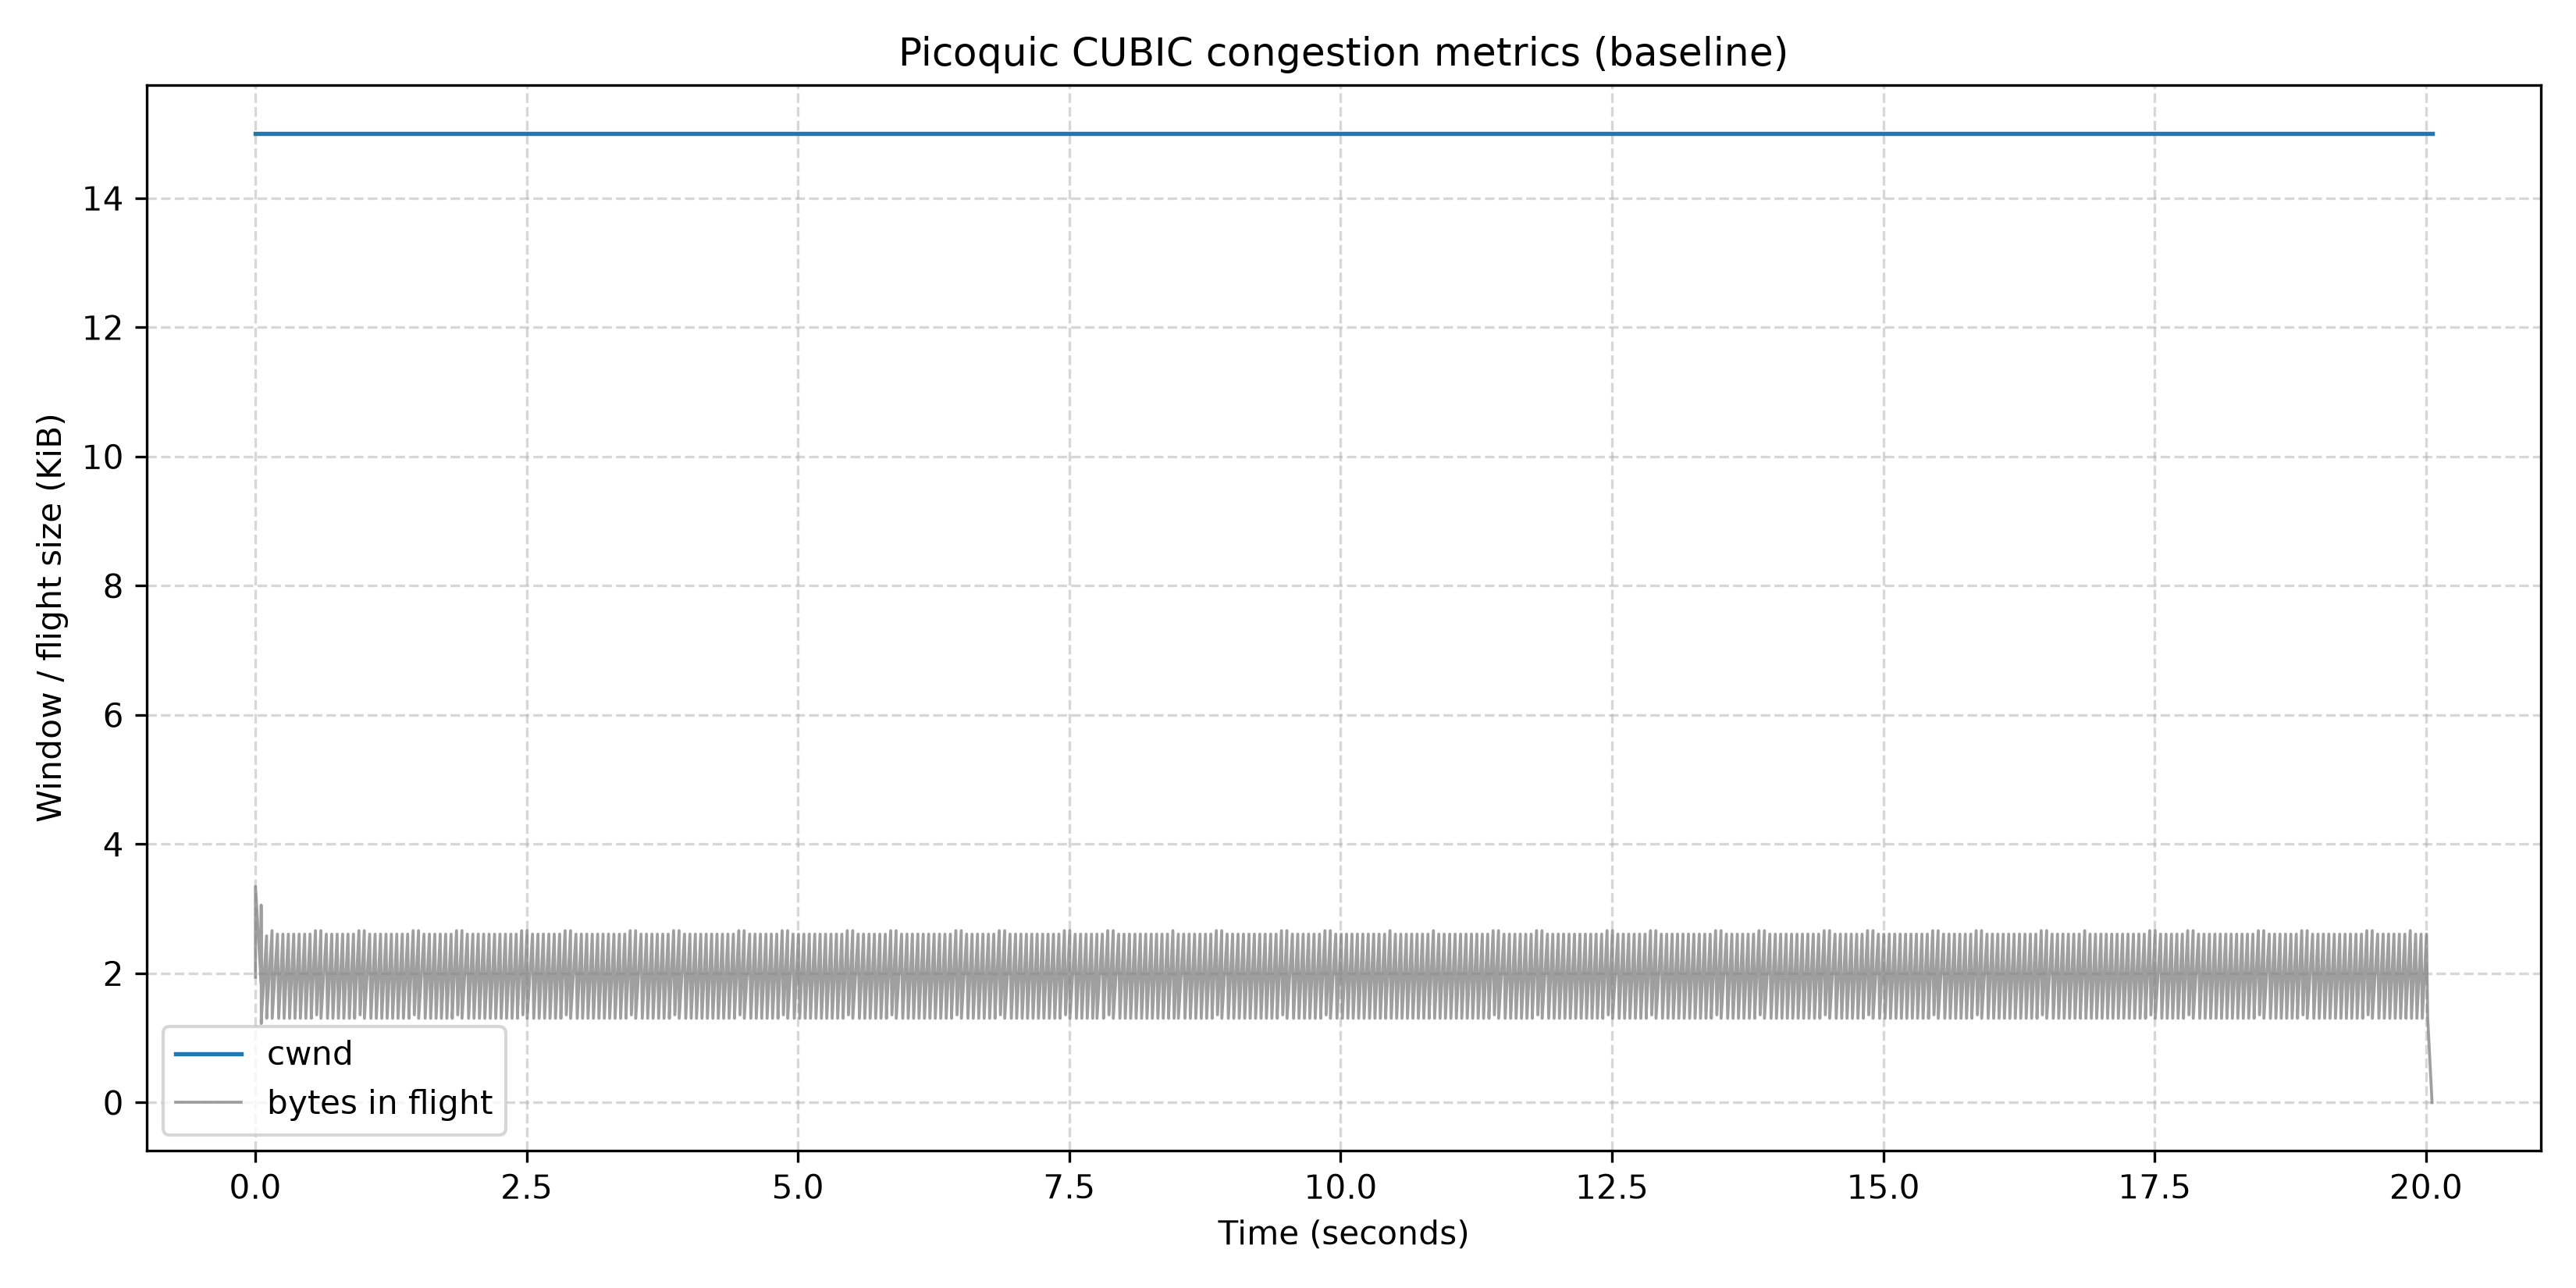
\includegraphics[width=0.92\textwidth]{plots/rate-limited-baseline-1.png}
\caption{Baseline: final cwnd 15.00 KiB; time-weighted mean 15.00 KiB; throughput 0.190 Mbit/s.}\end{figure}
\begin{figure}[H]\centering
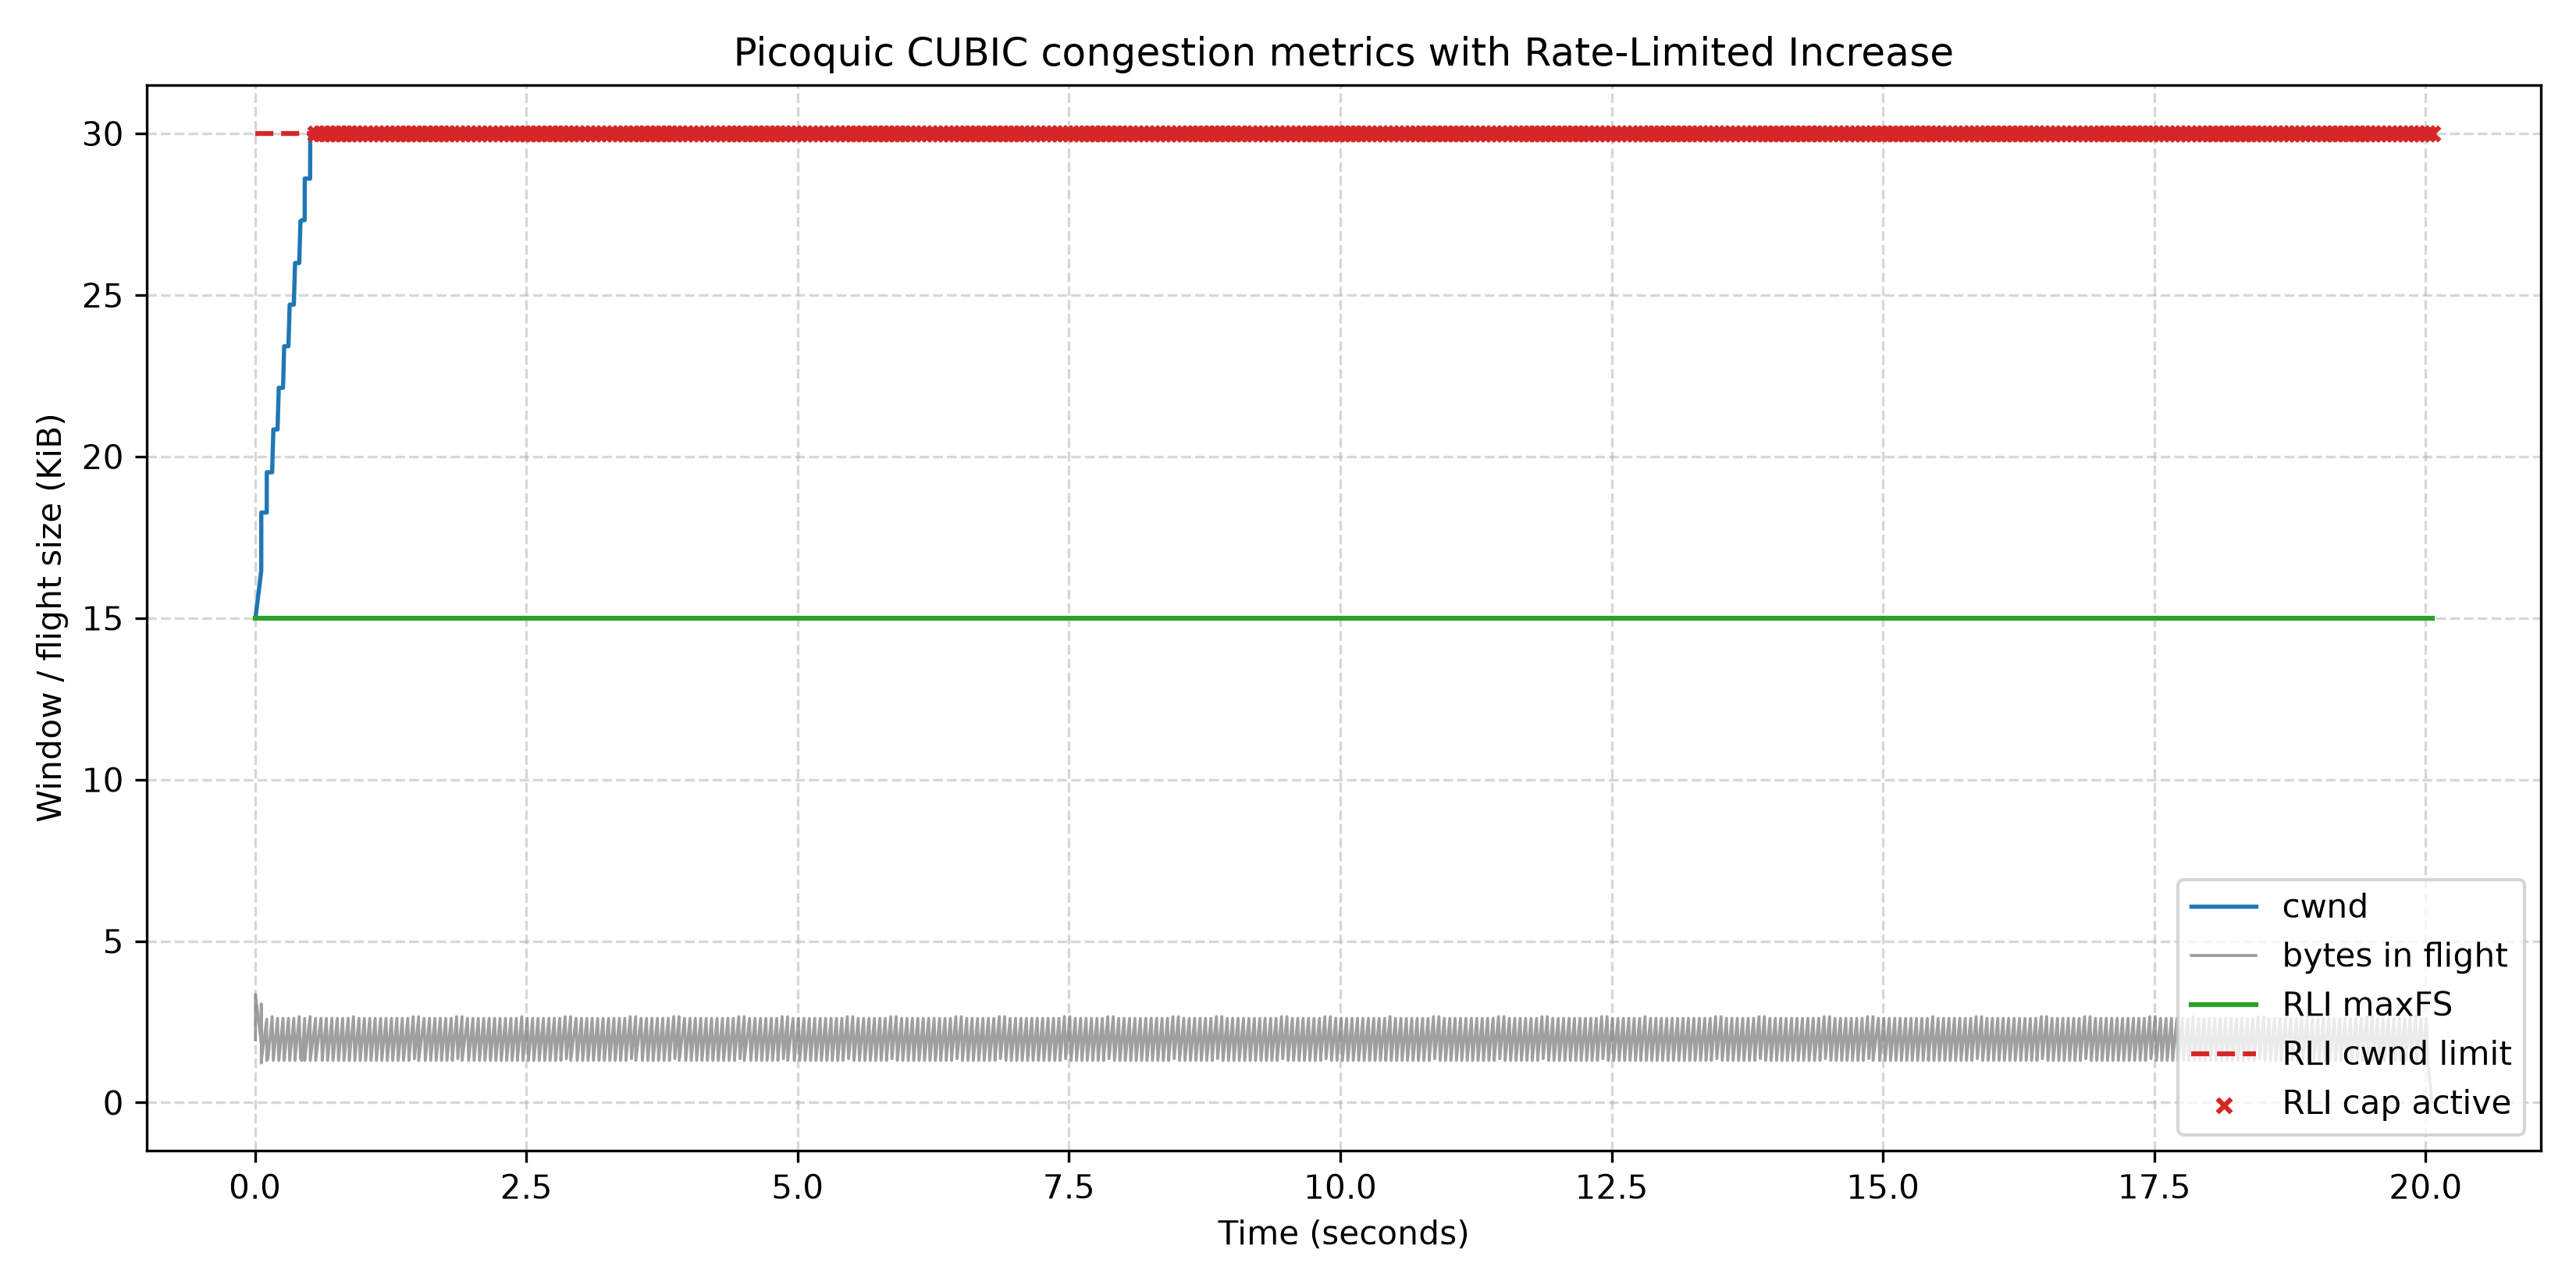
\includegraphics[width=0.92\textwidth]{plots/rate-limited-rli-1.png}
\caption{RLI: final cwnd 30.00 KiB; time-weighted mean 29.81 KiB; throughput 0.190 Mbit/s.}\end{figure}
RLI allows window growth up to its cap. The application supplies the same limited data in both runs.
\clearpage\subsection{Bulk control, repetition 1}
\begin{figure}[H]\centering
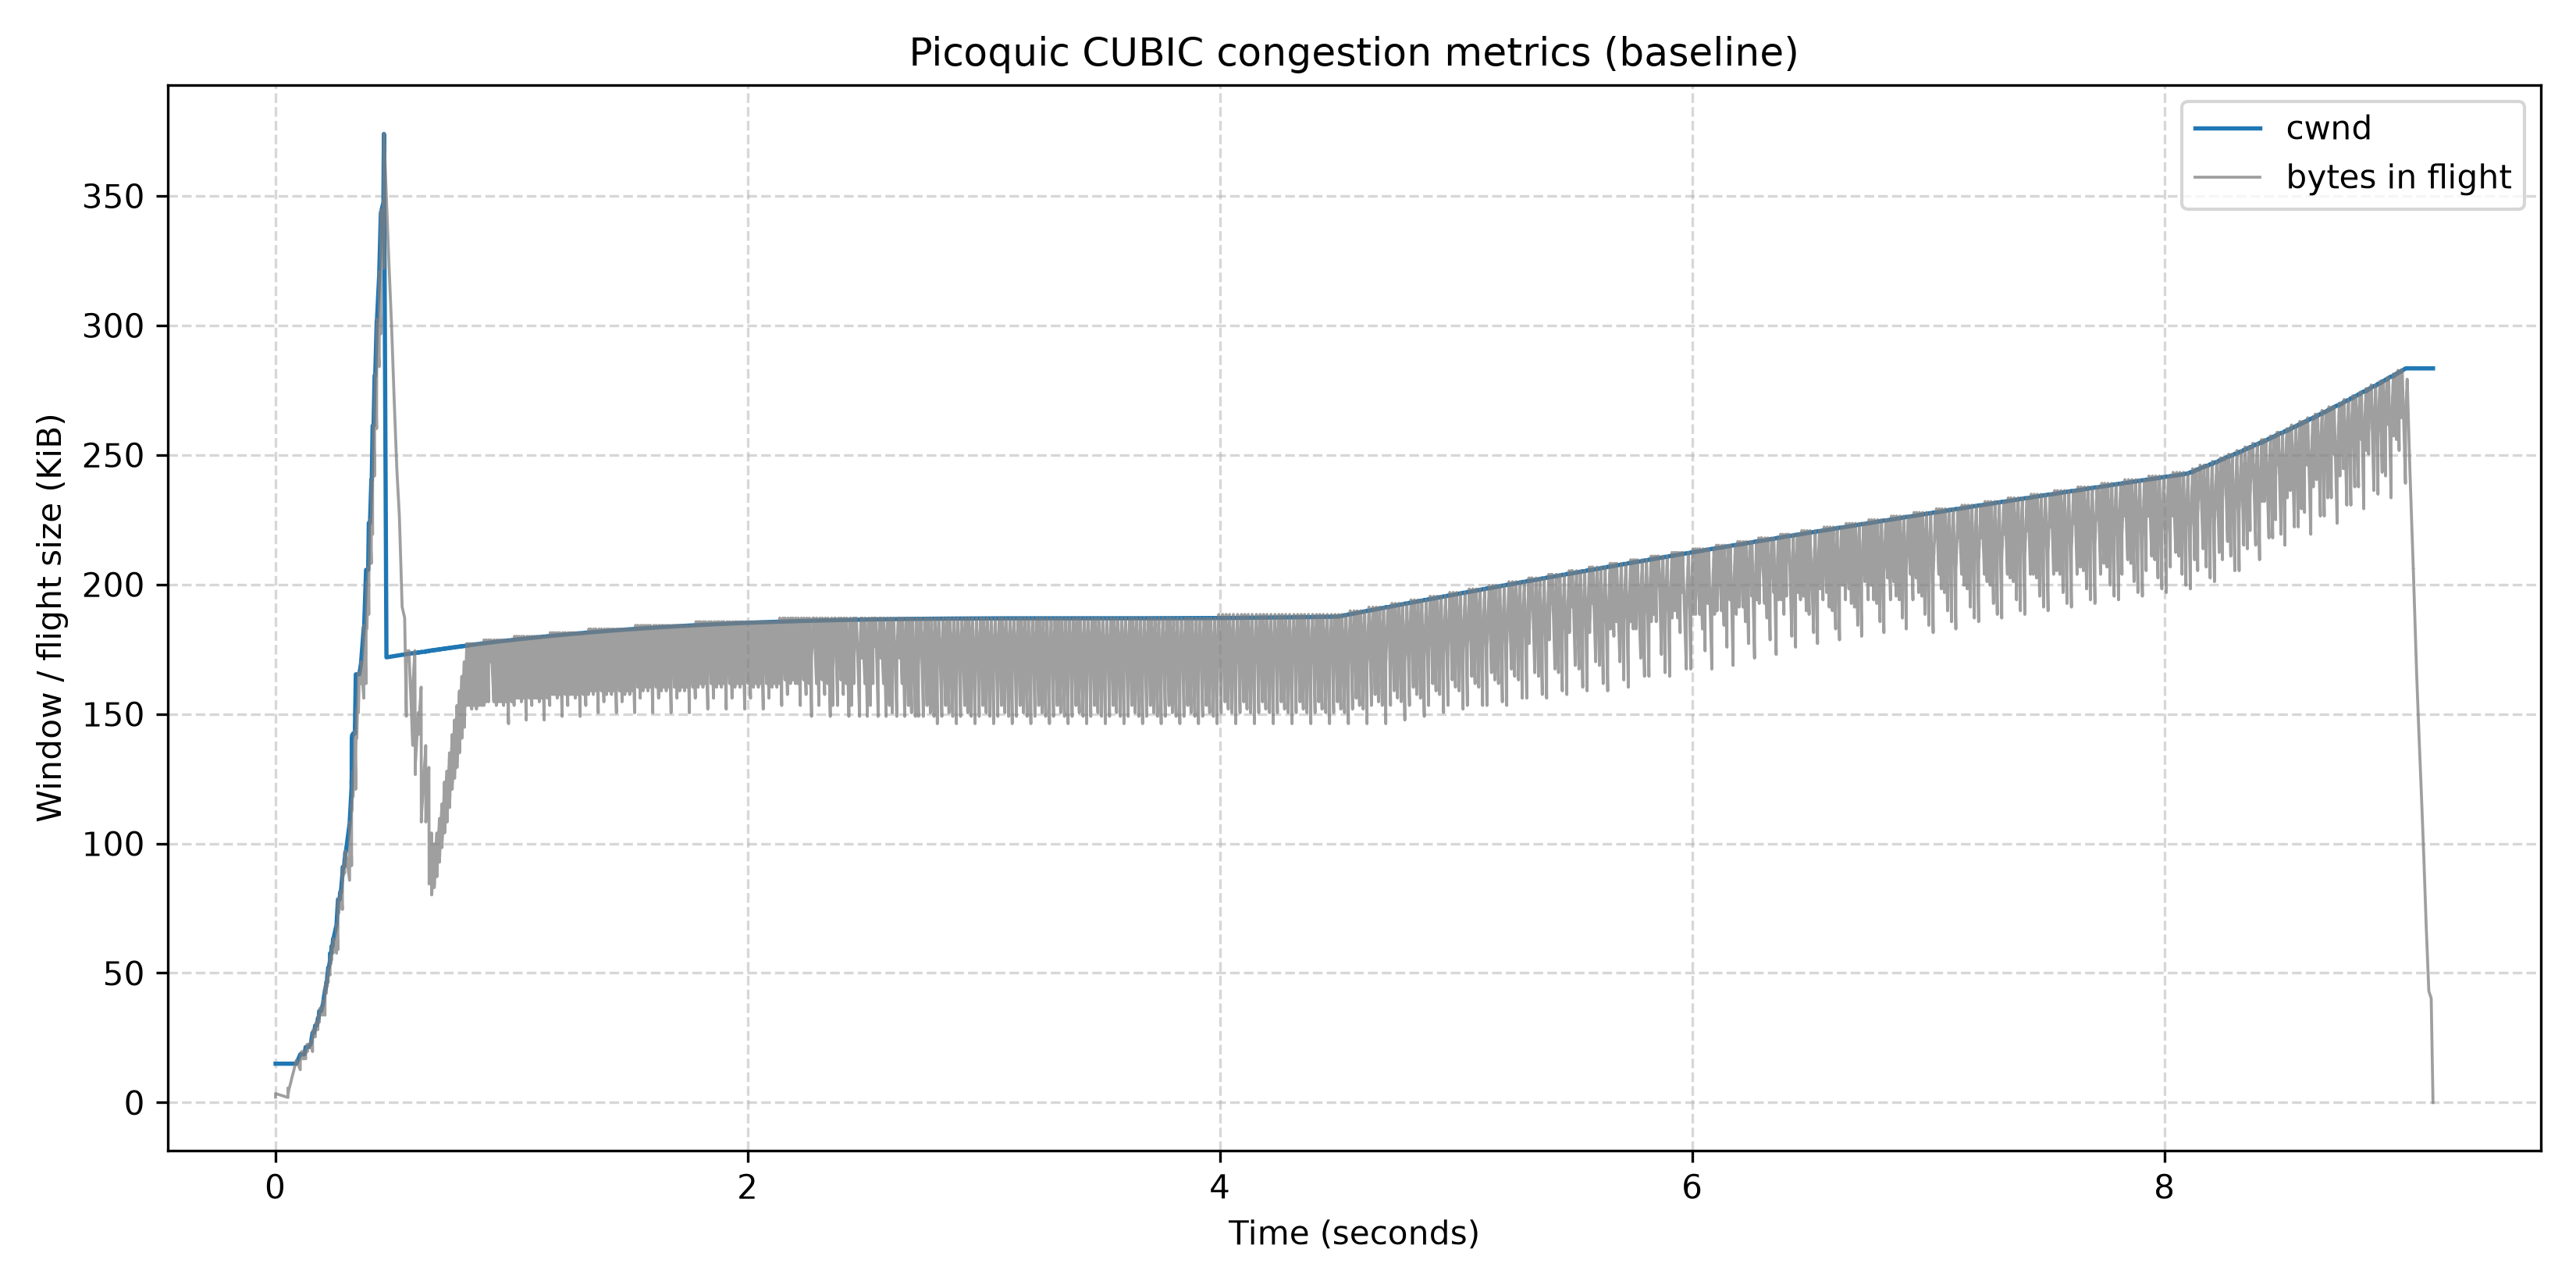
\includegraphics[width=0.92\textwidth]{plots/bulk-baseline-1.png}
\caption{Baseline: final cwnd 283.41 KiB; time-weighted mean 201.63 KiB; throughput 17.731 Mbit/s.}\end{figure}
\begin{figure}[H]\centering
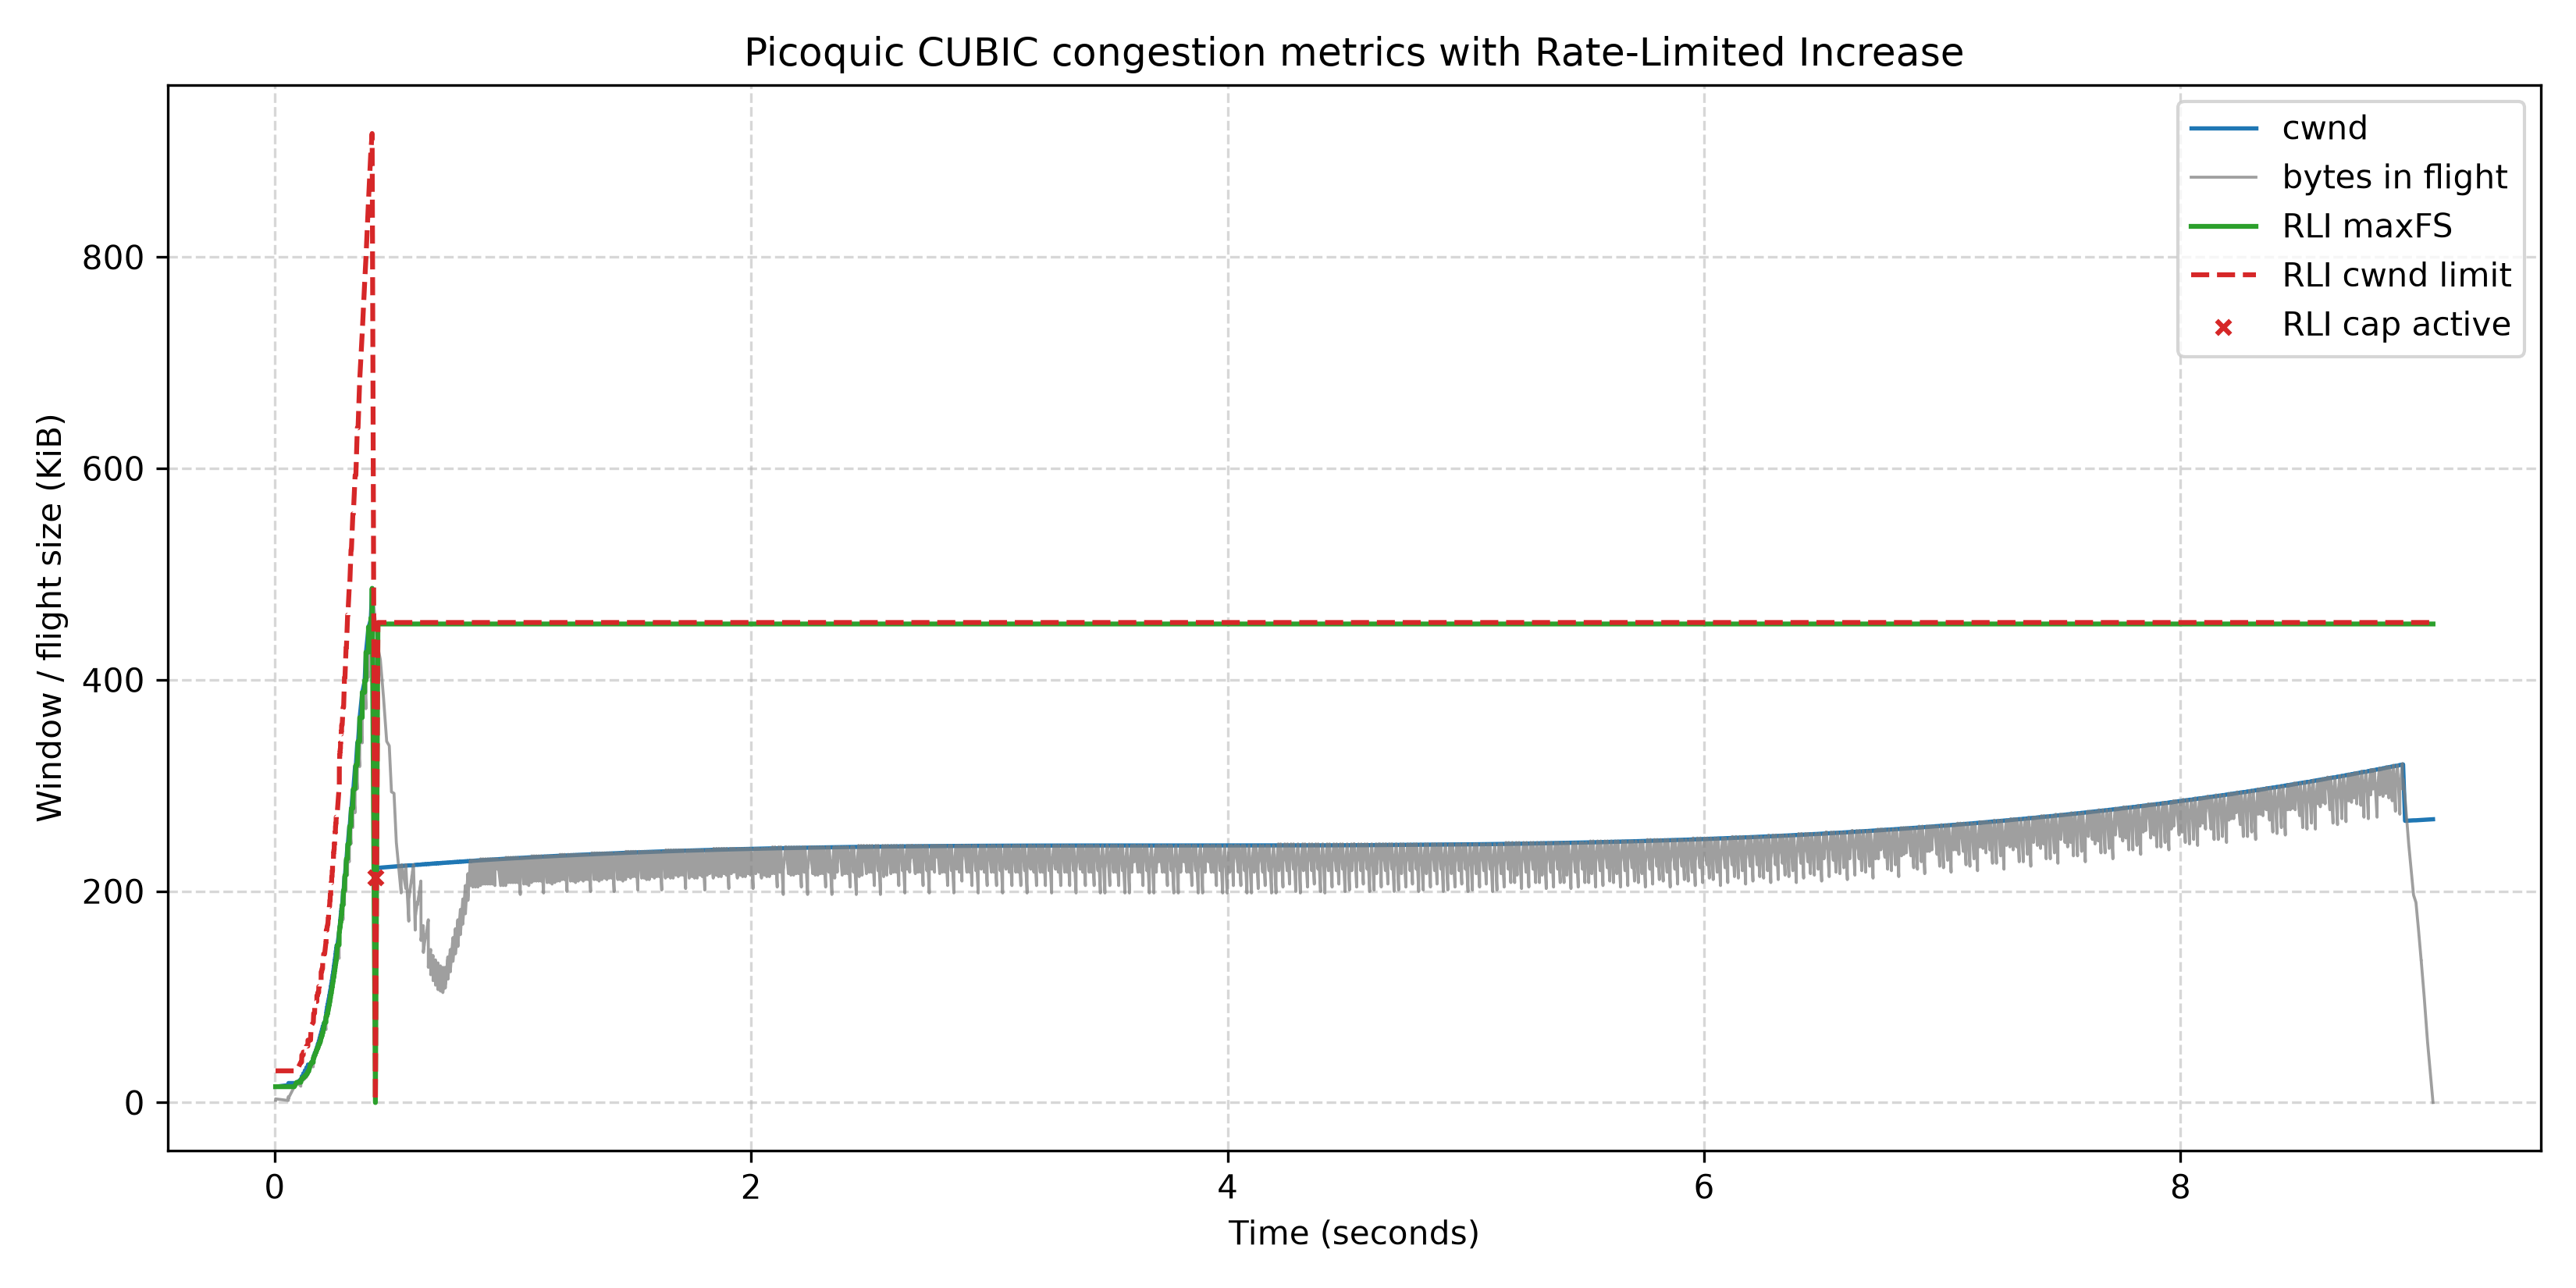
\includegraphics[width=0.92\textwidth]{plots/bulk-rli-1.png}
\caption{RLI: final cwnd 268.04 KiB; time-weighted mean 248.21 KiB; throughput 17.940 Mbit/s.}\end{figure}
Both senders have continuous data. Use the measured throughput to compare the runs; cwnd height alone does not show transfer speed.

\clearpage
\section{Competing-flow dumbbell graphs}
Each graph shows two simultaneous 20 MiB transfers across the same bottleneck.
This graph pair shows repetition 1.
The competing-flow results table uses means from all three repetitions.
\subsection{Two-flow dumbbell, repetition 1}
\begin{figure}[H]\centering
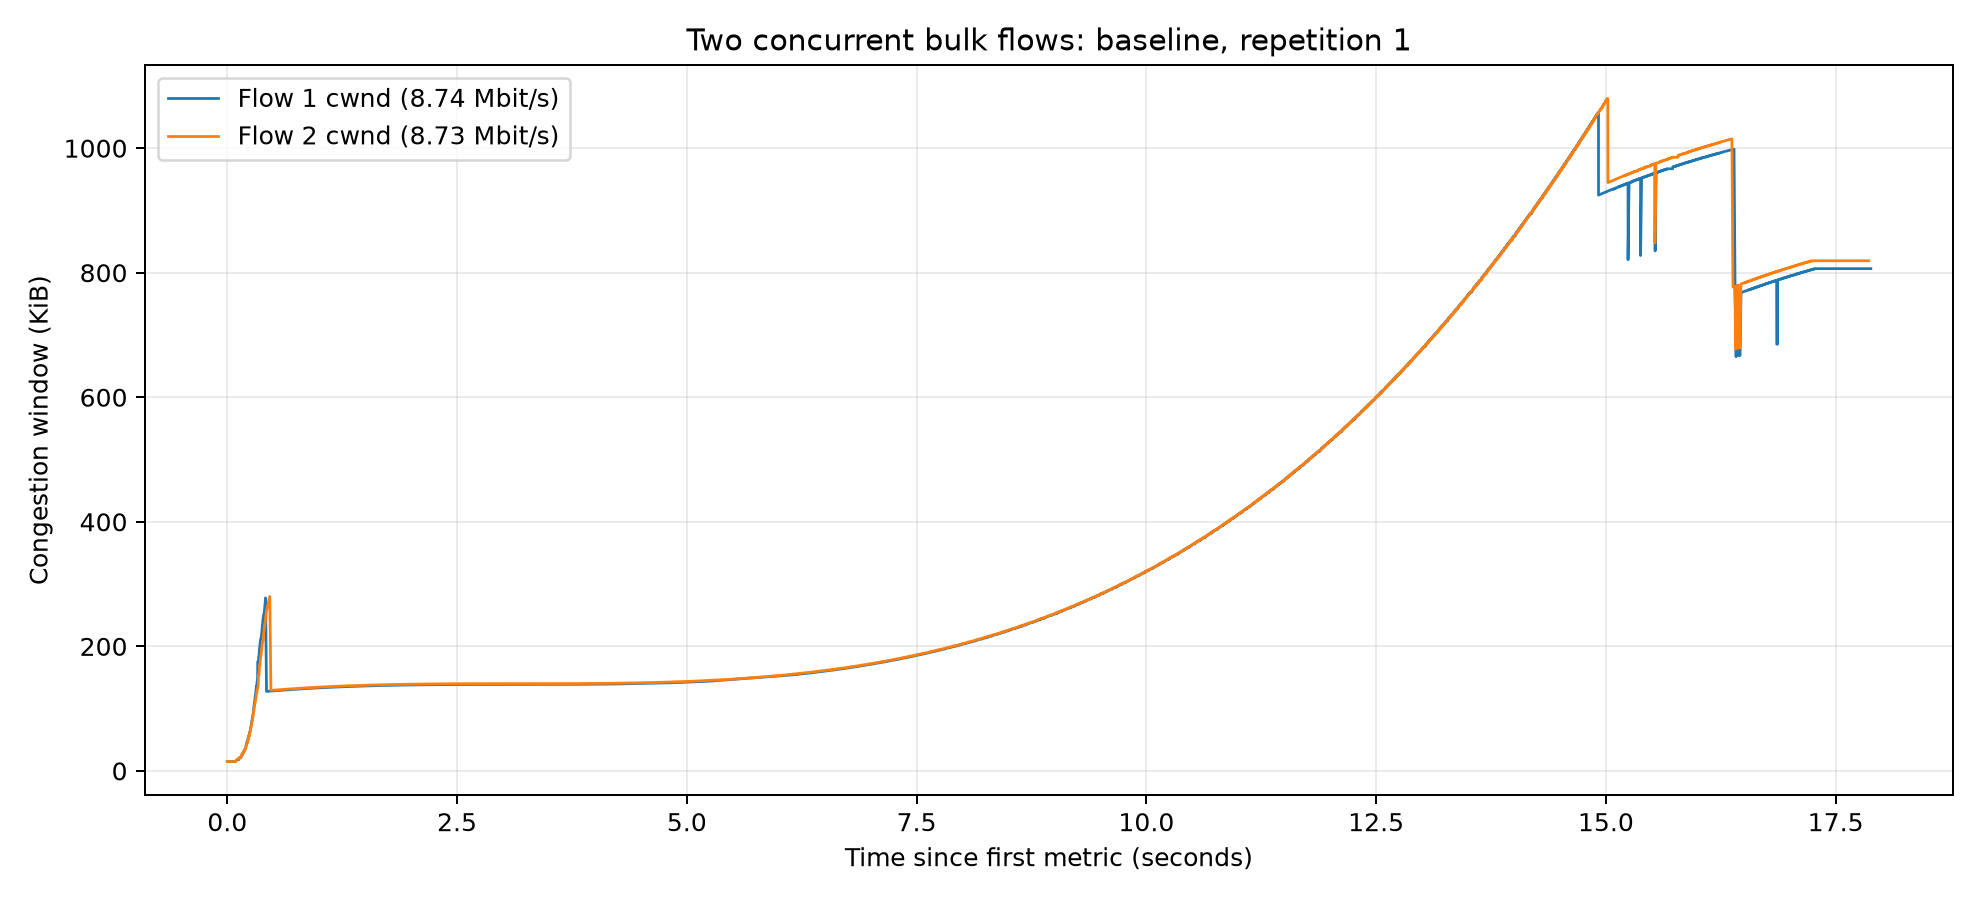
\includegraphics[width=0.92\textwidth]{plots/dumbbell/baseline-1.png}
\caption{Baseline: both client/server pairs transfer 20 MiB concurrently over the shared bottleneck.}\end{figure}
\begin{figure}[H]\centering
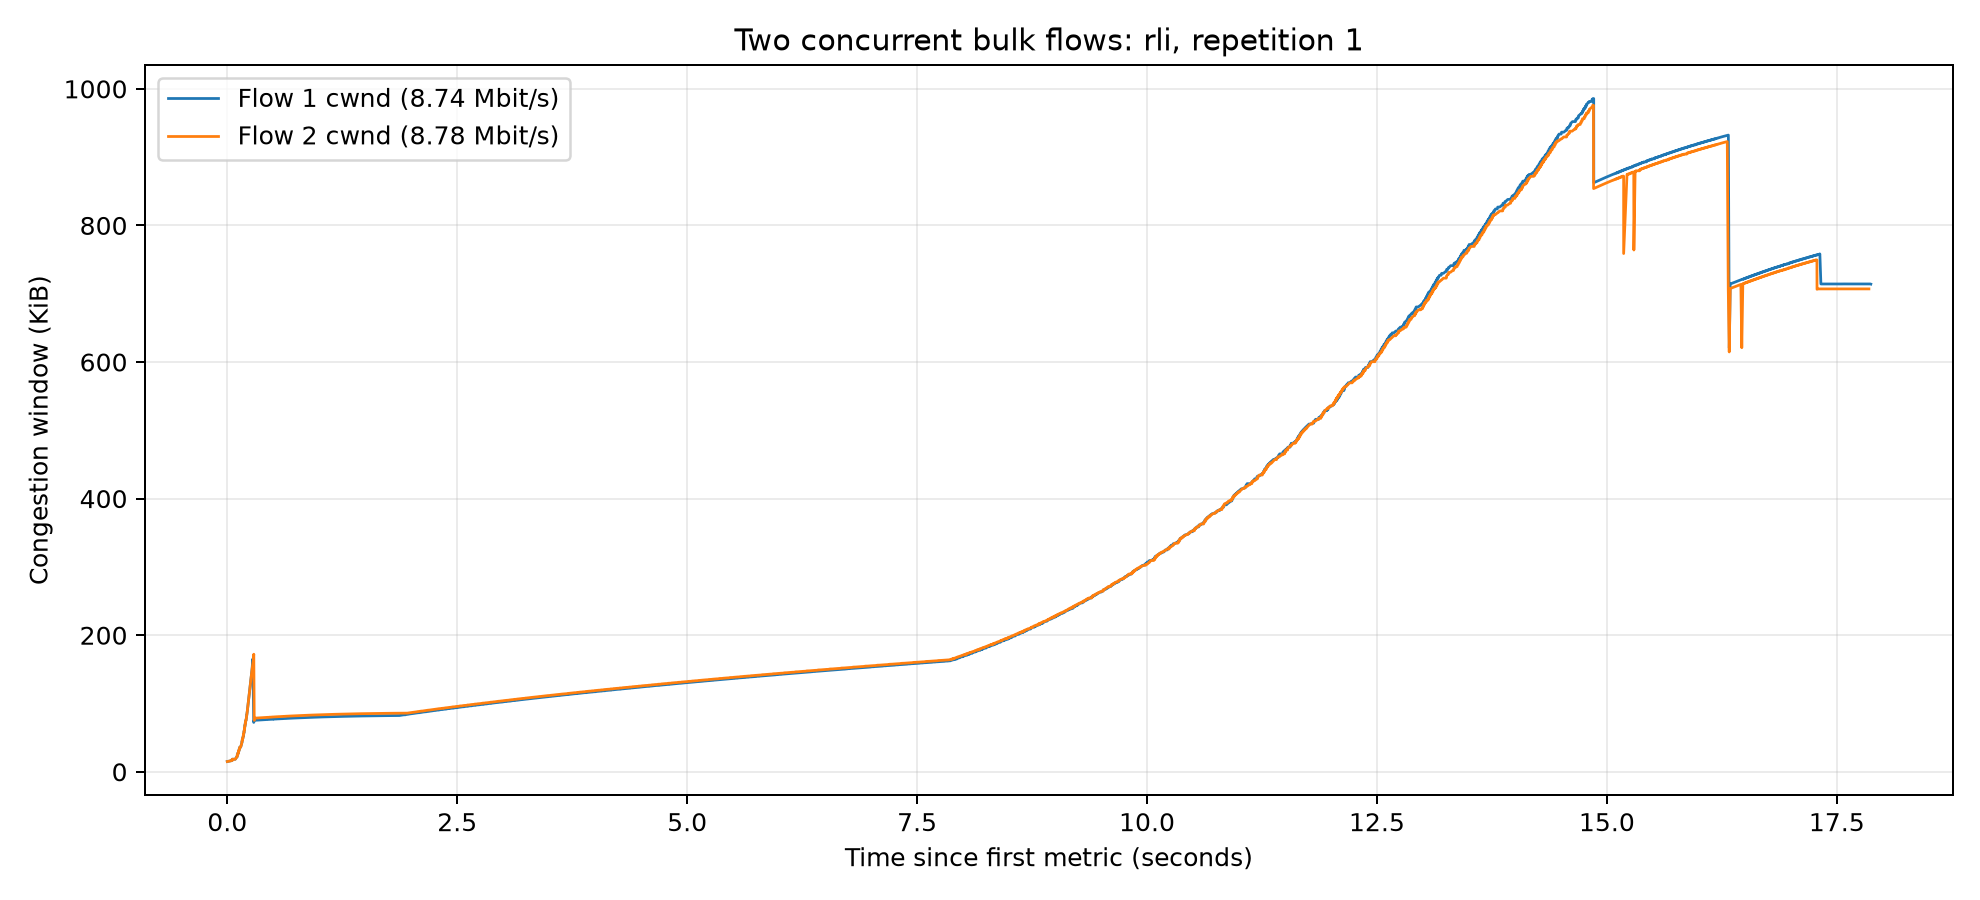
\includegraphics[width=0.92\textwidth]{plots/dumbbell/rli-1.png}
\caption{RLI: both client/server pairs transfer 20 MiB concurrently over the shared bottleneck.}\end{figure}
The lines show cwnd for the two competing flows. The results table gives their transfer rates and Jain index.

\end{document}
